\subsection*{Question 2.2}

In figure \ref{fig:q22} the four RMS errors for $\alpha$ in the
interval from 1--200. As the figure indicates the test data, have the
lowest error, and the first model have the best results, due to the
fact that it uses more features from the dataset to train the
model. The best value of $\alpha$ is one, since the error get bigger
the larger $\alpha$.

\begin{figure}[!htbp]
  \centering
  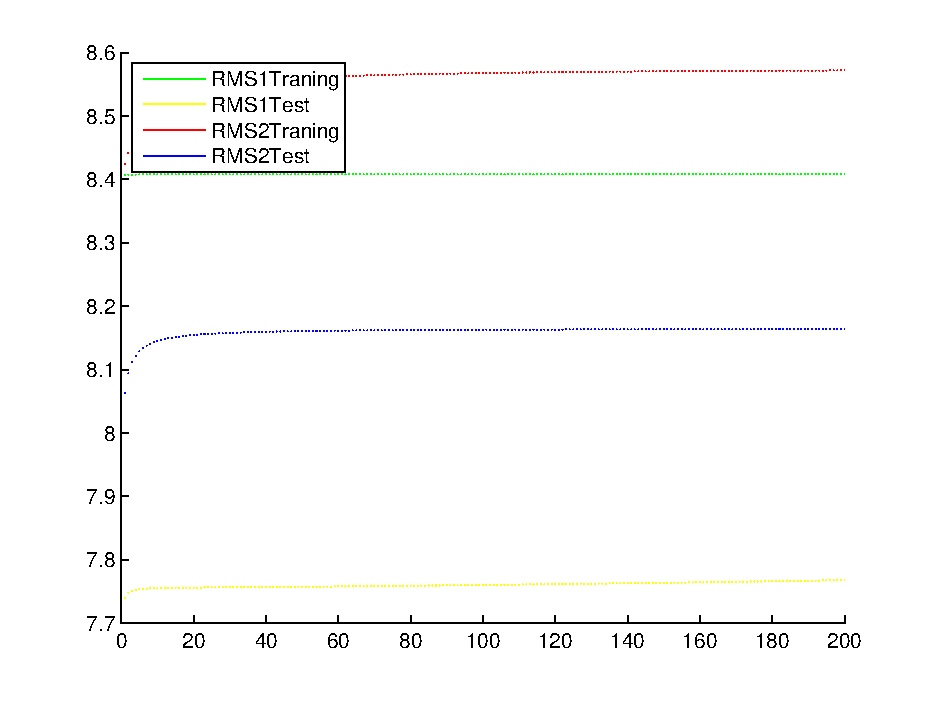
\includegraphics[width=0.75\textwidth]{./images/Q2.pdf}
  \caption{RMS for the two training models and test models}
  \label{fig:q22}
\end{figure}
